\begin{frame}[label=mc_conclusions]
    \frametitle{Simulating Meteor Radar Networks}
    \begin{columns}
        \begin{column}{0.7\textwidth}
            Monte Carlo simulation of meteor radar networks
            \begin{itemize}
                \item \alert{Provides insights into network performance} by investigating a representative population of meteors
                \item Simulations \alert{reveal the proportion and characteristics of unobserved meteors}%, giving an upper bound to how much counts can be improved 
                \item Helps \alert{inform what network improvements best supports science}
                \item The ability to closely re-create observations made by a real system shows its fidelity
            \end{itemize}
            \centering
            \begin{tcolorbox}[width = 6cm, center, boxrule=0pt,colback=yellow,arc=0pt,auto outer arc,left=0pt,right=0pt,boxsep=2pt]
                    \centering
                    \textbf{No other tools exist to investigate multistatic networks}
            \end{tcolorbox}
        \end{column}
        \begin{column}{0.4\textwidth}
            \centering
            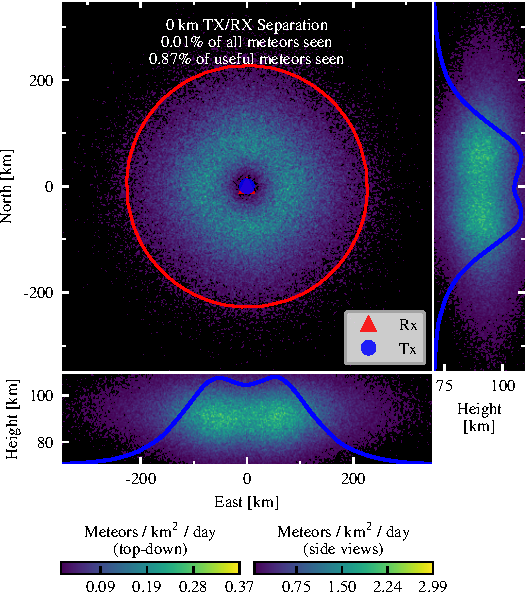
\includegraphics[width=\linewidth]{img/simulated_heatmap_0km.pdf}
        \end{column}
    \end{columns}
\end{frame}